% Драфт секции 3.3 — Результаты (MANGO / максимизация активации в ИНС)
% Источник: Pospelov2025, Neurocomputing
% Файл-источник: Disser/parts/neurotrain/main.tex, строки 408–570

\subsection{Сравнение с существующими методами максимизации активации}\label{sec:mango_performance}

Производительность методов оптимизации оценивалась по величине активации целевого нейрона в ответ на сгенерированные MEI. При большом количестве итераций подходы на основе разложения тензорного поезда продемонстрировали производительность несколько ниже, чем базовый метод Nevergrad Portfolio, который оказался наиболее эффективным среди рассмотренных безградиентных методов (рис.~\ref{nt:opt-conv}, таблица~\ref{table:am_methods}). Однако при малом и среднем количестве итераций, наиболее актуальных для реальных экспериментов, методы на основе TT показали сопоставимую или лучшую производительность. Все методы значительно превосходили базовый случайный поиск.

\begin{figure}[ht]
\centering
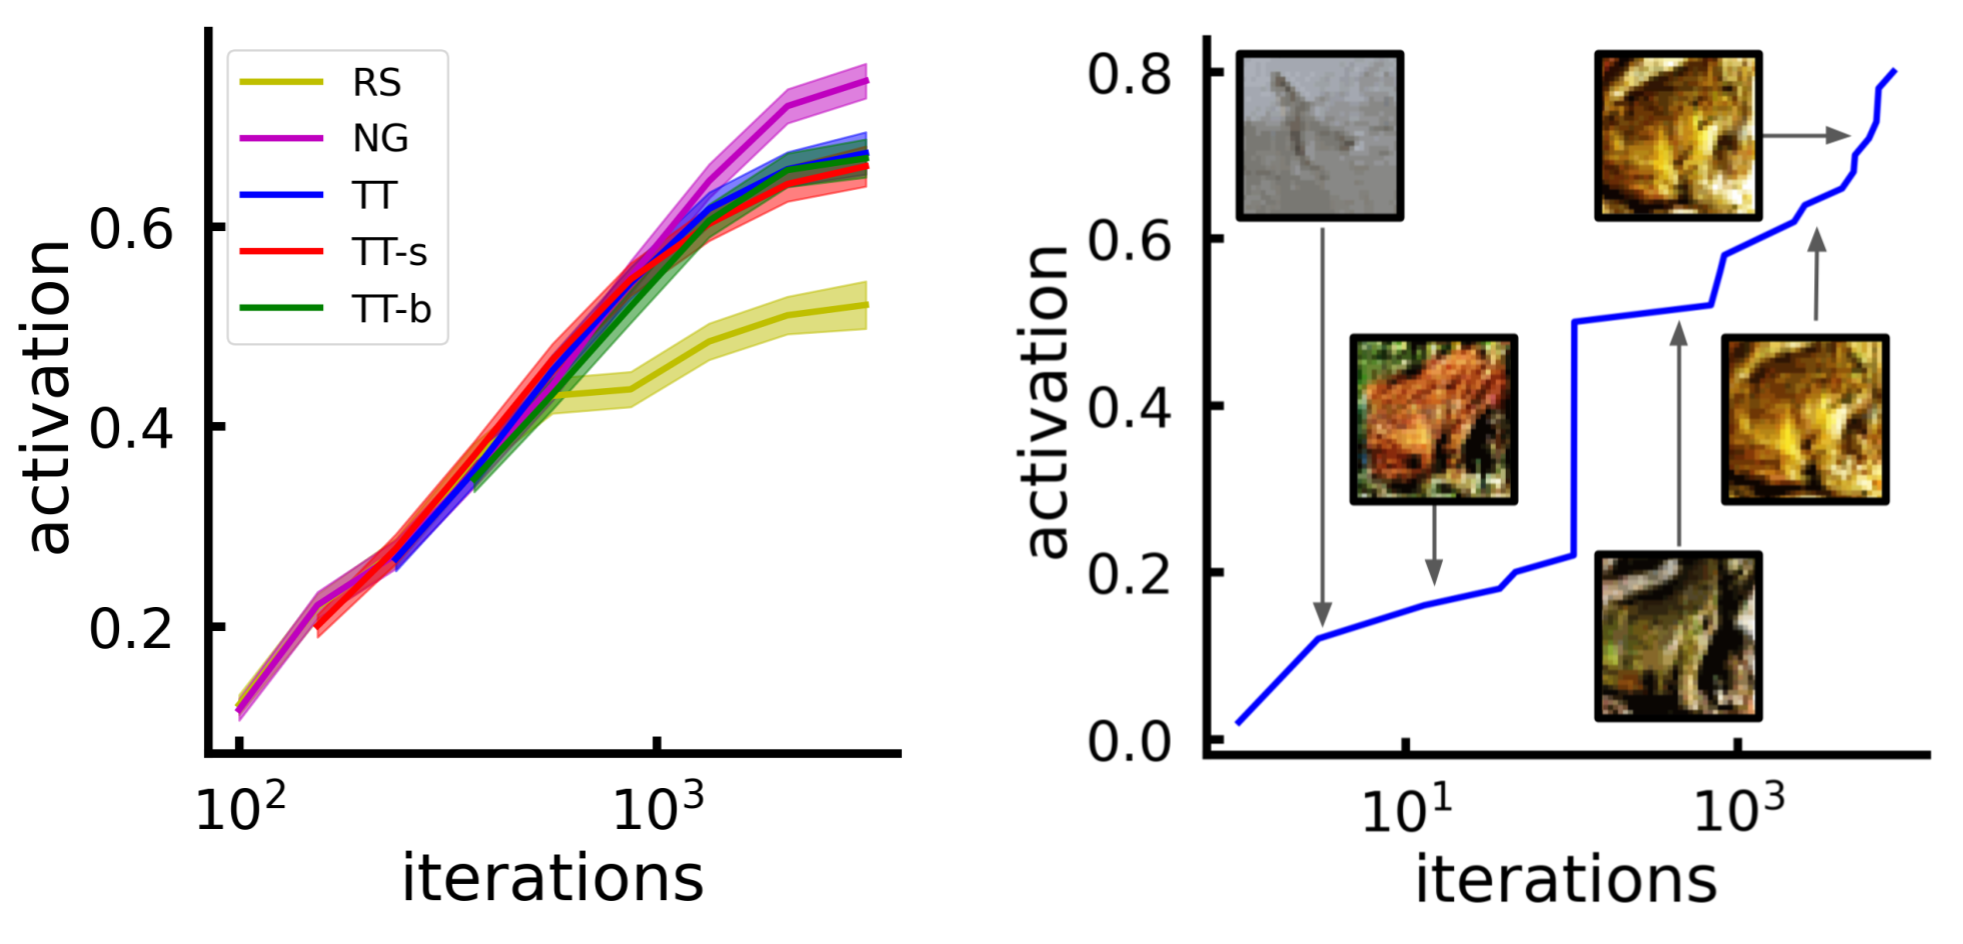
\includegraphics[width=0.98\textwidth]{images/neurotrain/fig4_new.png}
\caption{\textbf{Слева}: Активации нейронов для различных методов оптимизации, усредненные для всех единиц и слоев ИНС. Затененные области представляют стандартные ошибки. \textbf{Справа}: процесс формирования одного MEI на разных итерациях с соответствующими значениями активации.}
\label{nt:opt-conv}
\end{figure}

При этом было установлено, что метод PROTES в различных модификациях работает в 3--15 раз быстрее эталона Nevergrad Portfolio в зависимости от количества итераций, гиперпараметров и свойств изображения. Столь существенное преимущество в скорости делает методы на основе TT-разложения конкурентоспособными для практического применения.

Три различных тензорных метода и безградиентный эталон из библиотеки Nevergrad часто сходились к одним и тем же изображениям, что примечательно с учётом огромного числа возможных вариаций в латентном пространстве генератора. Это свидетельствует о том, что дискретные алгоритмы оптимизации действительно сходятся к хорошему оптимуму в латентном пространстве, а результаты могут быть обобщены на общее пространство изображений.

\begin{table}[ht]
\scriptsize
\centering
\begin{tabular}{|c|c|c|c|c|c|c|}
 \hline
 \multicolumn{7}{|c|}{Производительность методов оптимизации} \\
 \hline
~ & Акт. ($10^2$ ит.) &Акт. ($10^3$ ит.) & Акт. ($10^4$ ит.) & Время ($10^2$ ит.) &Время ($10^3$ ит.) & Время ($10^4$ ит.)\\
 \hline
 СП & $0.384\!\pm\!0.001$ & $0.468\!\pm\!0.001$ & $0.537\!\pm\!0.001$ & $10.202\!\pm\!0.033$ & $91.123\!\pm\!0.334$ & $861.266\!\pm\!3.176$  \\
 \hline
 NG & $0.393\!\pm\!0.001$ & $0.574\!\pm\!0.001$ & $\textbf{0.755}\!\pm\!\textbf{0.001}$ & $12.947\!\pm\!0.036$ & $163.45\!\pm\!0.294$ & $1685.464\!\pm\!3.04$ \\
 \hline
 TT & $0.411\!\pm\!0.001$ & $\textbf{0.581}\!\pm\!\textbf{0.001}$ & $0.675\!\pm\!0.001$ & $\textbf{3.267}\!\pm\!\textbf{0.006}$ & $14.456\!\pm\!0.007$ & $219.277\!\pm\!0.289$\\
 \hline
 TT-b & $\textbf{0.418}\!\pm\!\textbf{0.001}$ & $0.579\!\pm\!0.001$ & $0.662\!\pm\!0.001$ & $3.321\!\pm\!0.005$ & $\textbf{14.283}\!\pm\!\textbf{0.026}$ & $383.852\!\pm\!0.489$\\
 \hline
 TT-s & $0.392\!\pm\!0.001$ & $0.564\!\pm\!0.001$ & $0.679\!\pm\!0.001$ & $3.724\!\pm\!0.005$ & $15.236\!\pm\!0.007$ & $\textbf{127.406}\!\pm\!\textbf{0.173}$\\
 \hline
\end{tabular}
\caption{Средние MEI-связанные активации и время вычисления MEI для различных безградиентных методов оптимизации. Методы: СП~--- случайный поиск; NG~--- базовый Nevergrad Portfolio; TT, TT-b, TT-s~--- варианты оптимизации на основе разложения тензорного поезда.}
\label{table:am_methods}
\end{table}


\subsection{Динамика селективности индивидуальных нейронов в процессе обучения импульсной сети}\label{sec:mango_selectivity}

Для изучения динамики формирования MEI и их содержания были проанализированы оптимальные стимулы для импульсных слоёв сети ResNet18. Обучение проводилось в течение 1000 эпох, состояния сети записывались после каждой эпохи. Из девяти импульсных слоёв, равномерно распределённых между входным и выходным слоями, в каждом было отобрано 64 нейрона для построения MEI. Активация нейронов максимизировалась последовательно для всех 576 рассматриваемых нейронов тремя вариантами метода PROTES. В качестве генеративной модели использовался SN-GAN.

\paragraph{Энтропия классификации и формирование специализаций.}
Для количественной оценки селективности нейронов к конкретным классам полученные MEI подавались обратно в сеть, после чего вычислялась энтропия распределения вероятностей выходных классов, нормализованная относительно максимально возможной энтропии (для равномерного распределения по 10 классам CIFAR-10). Более равномерное распределение соответствует более абстрактным изображениям; высокая вероятность одного класса указывает на наличие соответствующего паттерна в MEI. Существуют и другие подходы к оценке селективности нейронов в ИНС~\cite{SNN-neuron-selectivity-Chevallier}.

\begin{figure}[ht]
\centering
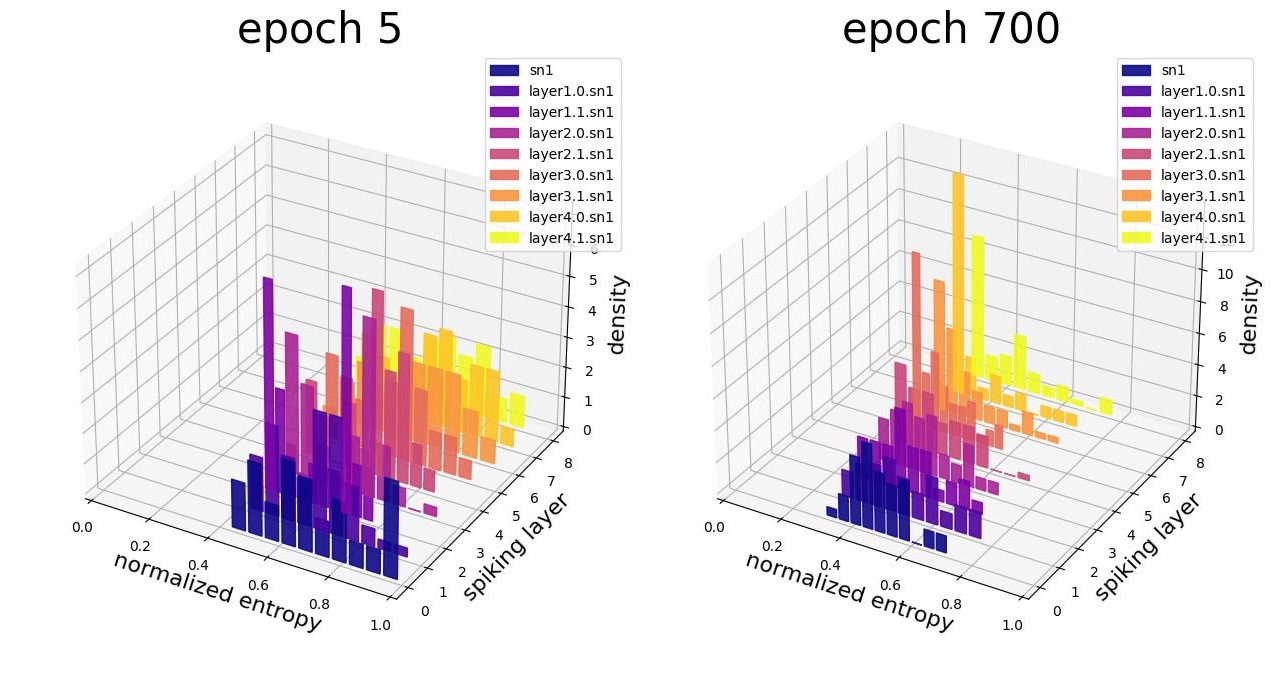
\includegraphics[width=0.9\textwidth]{images/neurotrain/entropies.jpg}
\caption{Распределение нейронов по энтропии вероятностей предсказания классов (меньшая энтропия = больше специализация на классе). \textbf{Слева}: ранняя стадия обучения (эпоха №5), \textbf{справа}: поздняя стадия обучения (эпоха №700).}
\label{nt:layer_spec}
\end{figure}

Результаты представлены на рис.~\ref{nt:layer_spec}. В последних импульсных слоях обученной модели наблюдался резкий пик MEI с низкой энтропией, что свидетельствует о высокой уверенности модели при классификации MEI. Даже в середине сети большинство нейронов уже оказались специфически связаны с определённым классом. Напротив, на ранней стадии обучения какая-либо специфичность MEI для конкретного класса отсутствовала.

Процесс формирования MEI, как правило, состоял из двух стадий. На первой стадии оптимизация проходила в латентном пространстве почти случайным образом при низкой уверенности классификации сети. Затем процесс сходился к определённому MEI, а дальнейшая оптимизация лишь уточняла его. Переход между стадиями сопровождался резким увеличением уверенности классификации, особенно для MEI, напоминающих обучающие изображения чётко различимых классов (рис.~\ref{nt:opt-conv}).

\paragraph{Критерий селективности.}
Три метода на основе TT-разложения часто сходились к похожим изображениям. С учётом высокой сложности ландшафта потенциальных MEI был использован следующий составной критерий селективности нейрона к конкретному классу:
\begin{itemize}
    \itemsep0em
    \item \textbf{Стабильность}: все три метода максимизации сходились на изображениях одного и того же класса (класс MEI определялся по максимальной вероятности на выходе сети).
    \item \textbf{Уверенность}: вероятность лучшего класса составляла не менее 75\%.
    \item \textbf{Активация}: активность целевого нейрона составляла не менее 75\% от максимально возможной (активность вычислялась суммированием количества импульсов по всем каналам для данного нейрона).
\end{itemize}

\begin{figure}[ht]
\centering
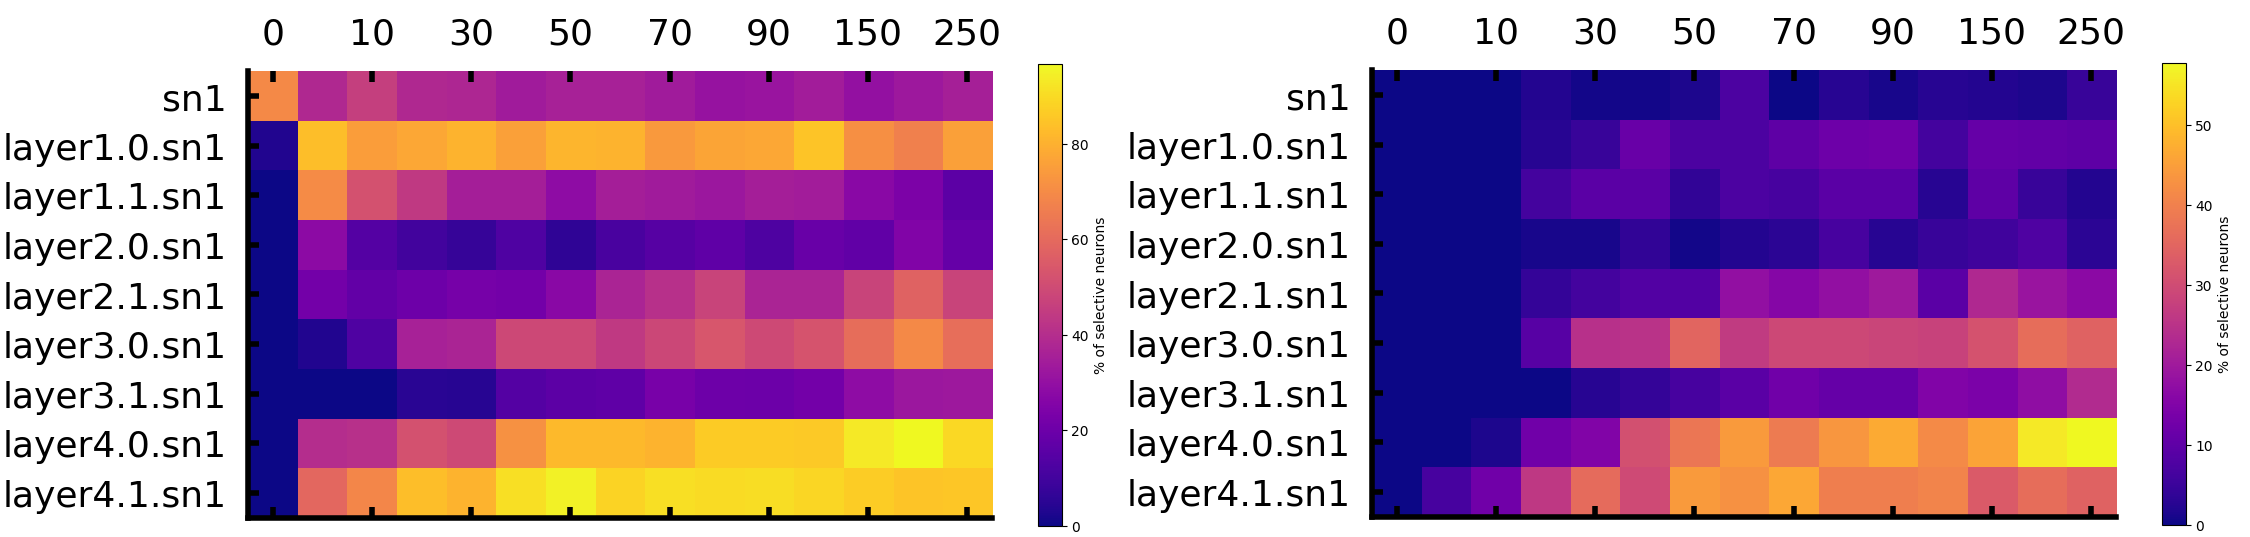
\includegraphics[width=0.95\textwidth]{images/neurotrain/fraction-of-selective-neurons.png}
\caption{{Доля селективных нейронов. Горизонтальная ось~--- номер эпохи, вертикальная ось~--- слои (ниже = глубже). \textbf{Слева}: порог активации~--- импульсы $\geq$75\% времени экспозиции; \textbf{Справа:} дополнительно максимальная вероятность класса $\geq$75\%, с максимальным классом, стабильным при различных методах максимизации.}}
\label{nt:fraction-of-selective-neurons}
\end{figure}

Подавляющее большинство специализированных нейронов обнаружено в конечных слоях модели, где MEI содержали наиболее сложные паттерны (рис.~\ref{nt:fraction-of-selective-neurons}). Вместе с тем значительное количество нейронов, связанных с определённым классом, было выявлено и в промежуточных слоях --- до 40\% от общего числа. Высокоселективные нейроны были обнаружены уже в третьем импульсном слое.

\paragraph{Динамика активаций в процессе обучения.}
По мере обучения модели количество высокоспециализированных нейронов увеличивалось. Для количественной оценки «качества» MEI был вычислен усреднённый нейронный отклик на MEI по слоям и эпохам обучения. Результаты представлены на рис.~\ref{nt:image-acts} и~\ref{nt:activation-dynamics}. В целом MEI-связанная активность в последних слоях возрастала с обучением, хорошо коррелируя с производительностью модели (рис.~\ref{nt:activation-dynamics}, справа). Для промежуточных слоёв MEI-связанная активность достигала плато и могла показывать небольшое снижение на поздних эпохах. При этом наблюдалось аномально позднее развитие MEI в предпоследних слоях сети (слой 3.1), что сопровождалось более слабой активацией целевых нейронов (рис.~\ref{nt:image-acts}, справа). Возможным объяснением этого эффекта является продолжающаяся реструктуризация MEI в указанных слоях, выполняющих роль «шлюза» к более глубоким специализированным слоям.

\begin{figure}[ht]
\centering
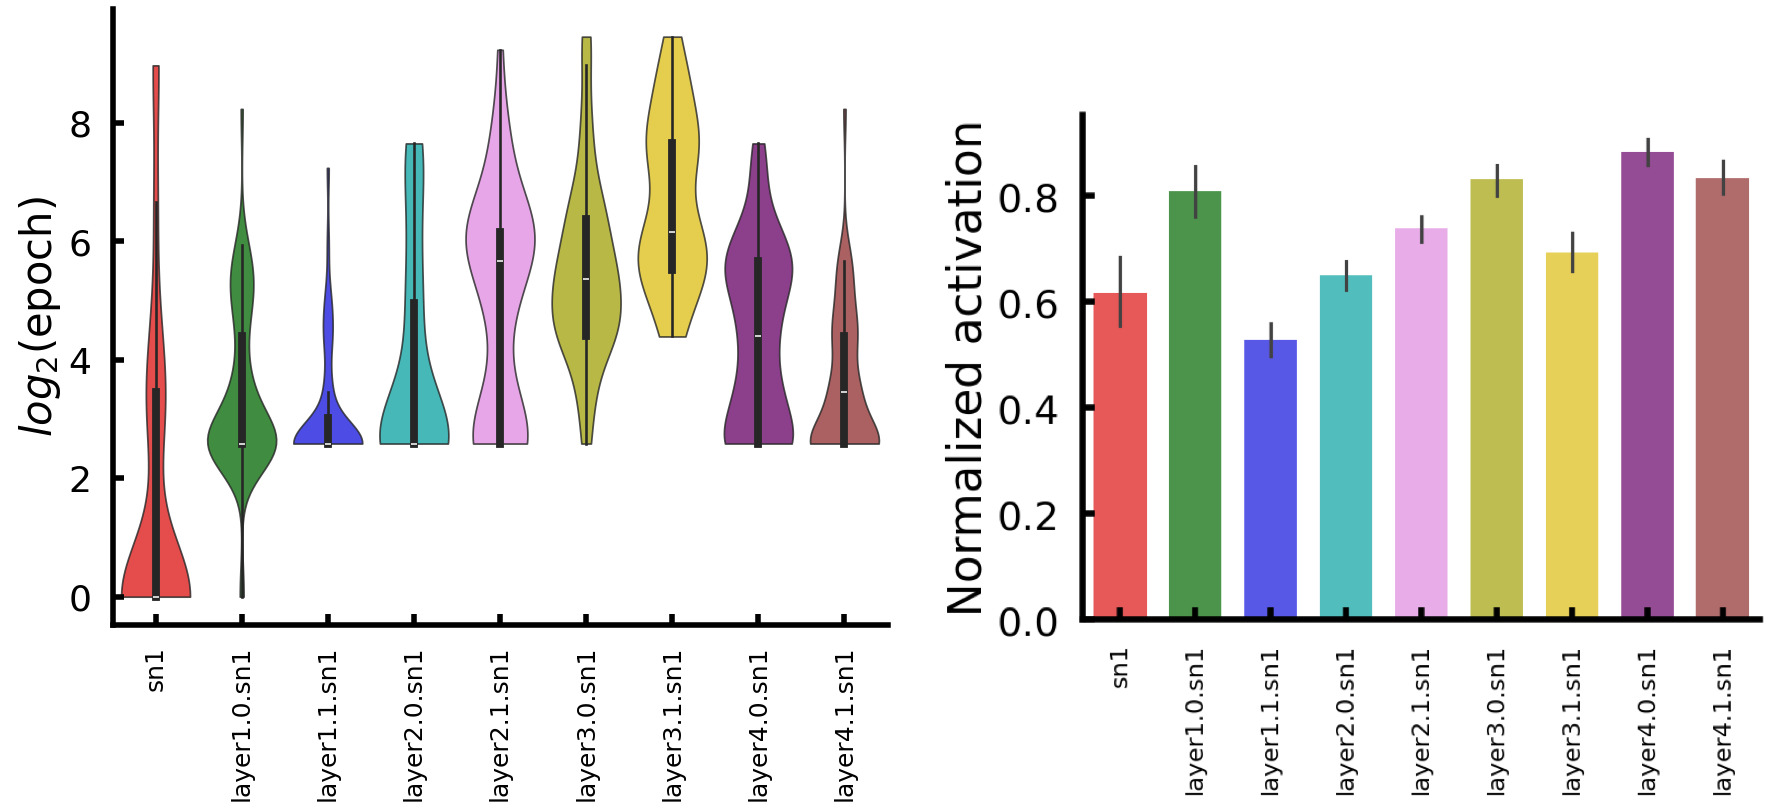
\includegraphics[width=0.95\textwidth]{images/neurotrain/emergence-of-specializations.png}
\caption{
Возникновение нейронных специализаций. Горизонтальная ось~--- глубина слоя (увеличивается слева направо). \textbf{Слева}: распределение (по нескольким запускам) номеров первых эпох, когда появляется сильный MEI (импульсы нейрона $\geq$75\% времени экспозиции). \textbf{Справа}: нормализованная активация от MEI (планки погрешностей~--- 95\% доверительный интервал).}
\label{nt:image-acts}
\end{figure}

\begin{figure}[ht]
\centering
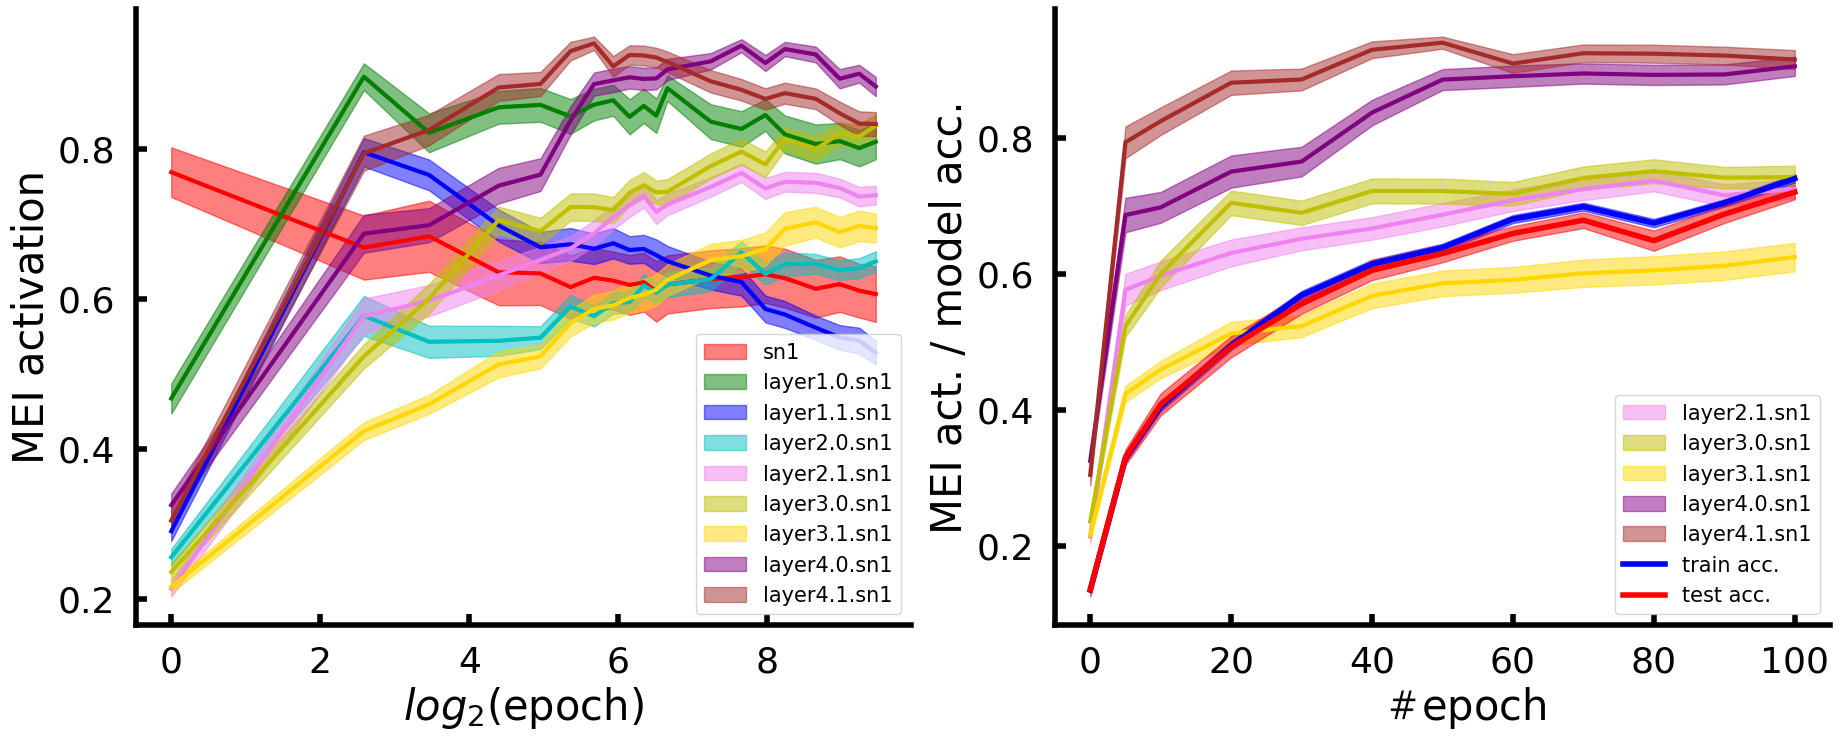
\includegraphics[width=0.95\textwidth]{images/neurotrain/activation-dynamics.png}
\caption{{\textbf{Слева}: динамика активаций нейронов в ответ на их MEI. \textbf{Справа}: то же самое для первых 100 эпох с точностью классификации модели на тех же осях.}}
\label{nt:activation-dynamics}
\end{figure}

\paragraph{Лабильные нейроны.}
Отдельного рассмотрения заслуживают «лабильные» нейроны, изменяющие свою селективность по мере обучения. Для их выявления отслеживались нейроны, соответствовавшие критериям специализации более чем на одном классе в ходе обучения. Такие нейроны представляют интерес, поскольку помогают понять механизмы формирования «узких» специализаций и часто оказываются специализированными на абстрактных концепциях, которые могут служить строительными блоками для классификации более сложных паттернов.

\begin{figure}[ht]
\centering
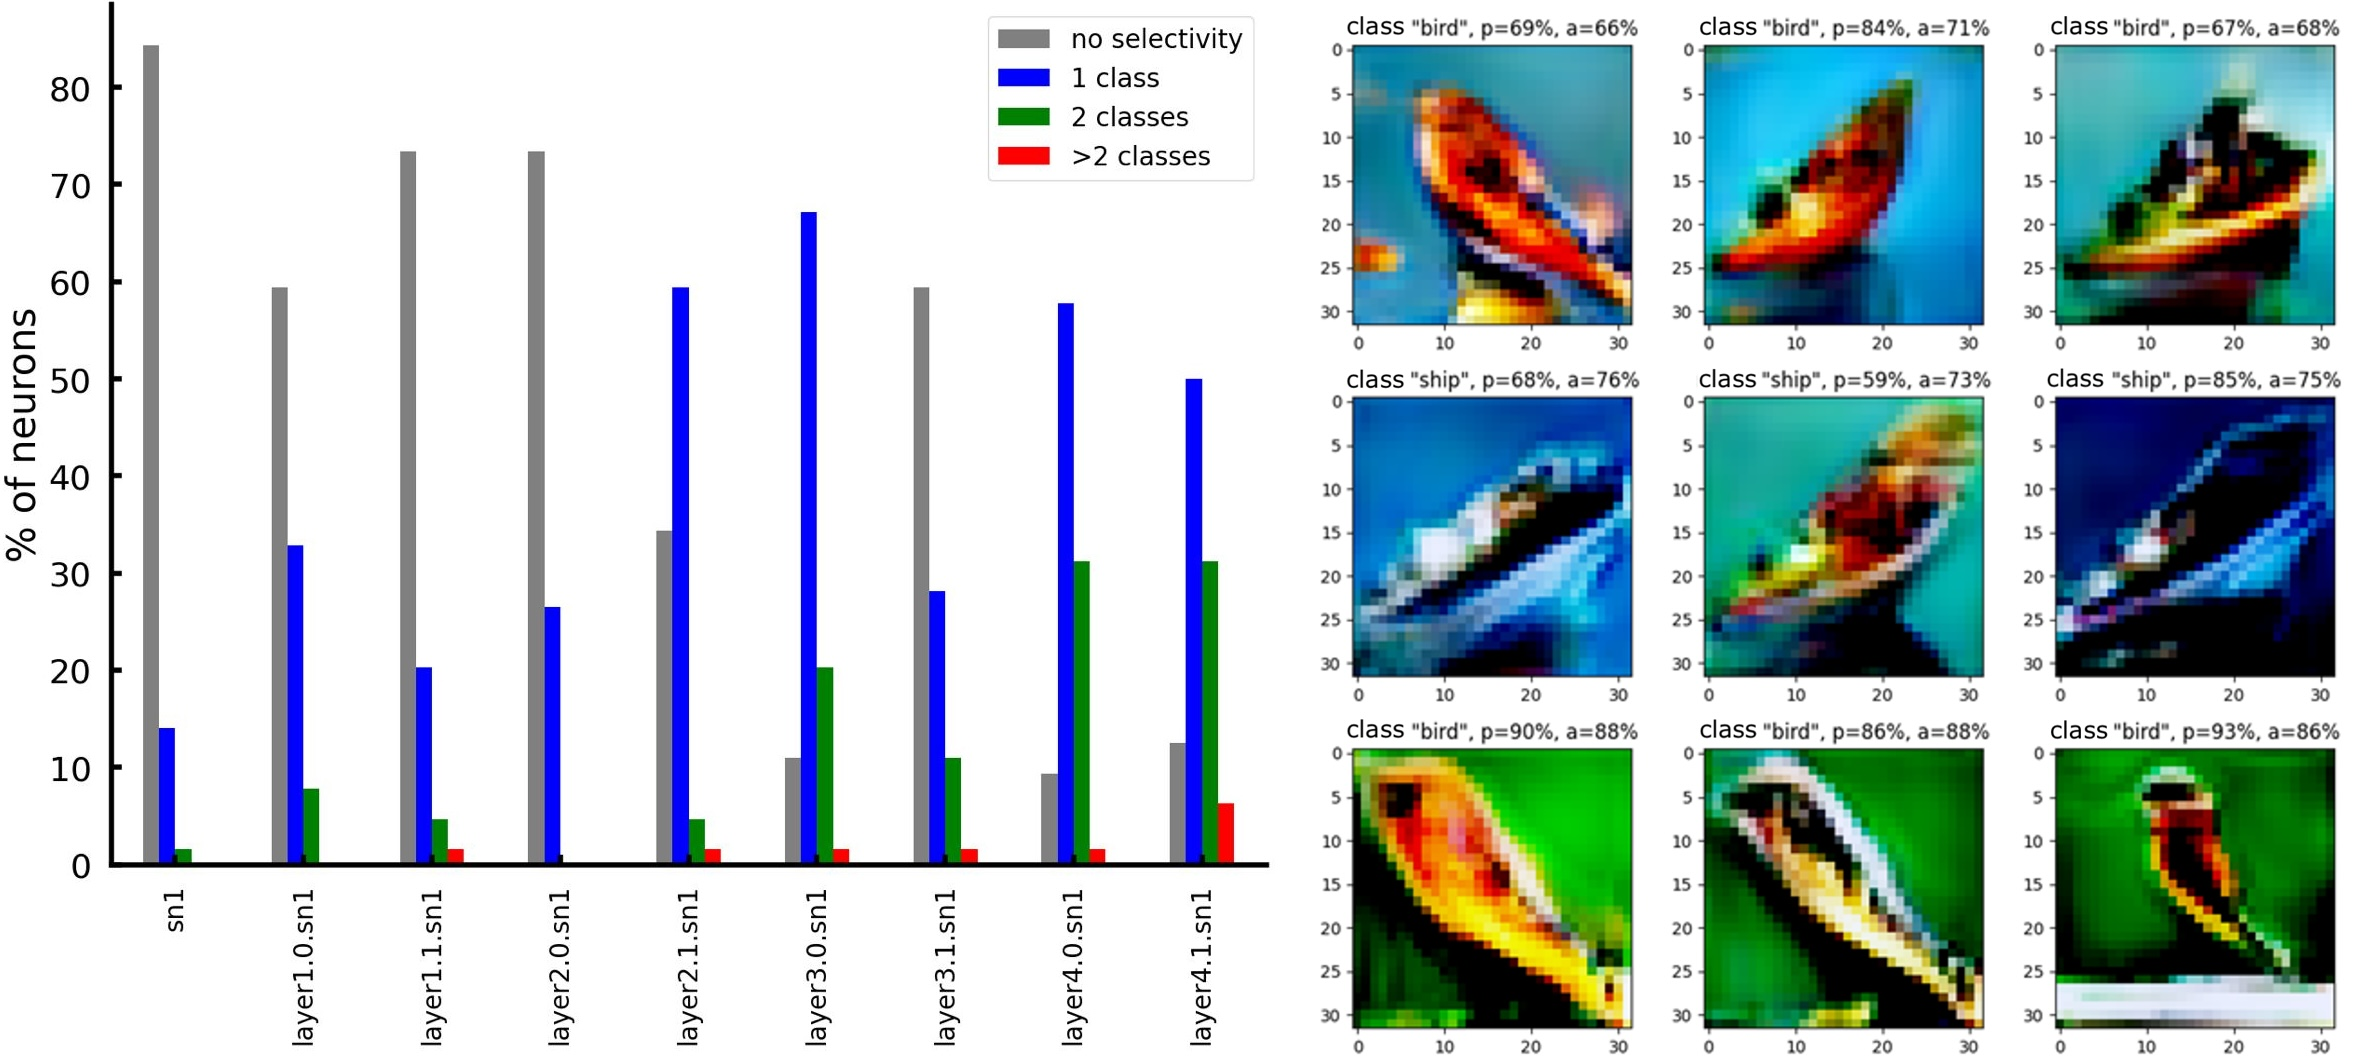
\includegraphics[width=1.0\textwidth]{images/neurotrain/by_1-2-many_specializations_and-bird-ships.jpg}
\caption{\textbf{Слева:} доли неспециализированных, стабильных (селективных только к 1 классу) и лабильных (селективных к 2 или более) нейронов в зависимости от глубины слоя. \textbf{Справа:} осциллирующие MEI лабильного \textbf{\textit{нейрона «птица-корабль»}}, \textbf{строки}: эпохи №~40, 100, 300 обучения; \textbf{столбцы:} результаты, полученные методами оптимизации TT, TT-S, TT-B. Подписи над каждым MEI содержат информацию о преобладающем классе согласно результатам классификации, вероятности и активации нейрона в процентах от максимально возможной.}
\label{nt:labile-neurons-distr-and-bird-ship}
\end{figure}

Характерный пример представлен на рис.~\ref{nt:labile-neurons-distr-and-bird-ship} (справа): нейрон селективно активируется на вытянутых, диагонально расположенных структурах на сине-зелёном фоне. В этой области латентного пространства вложения классов «птица» и «корабль» оказываются близкими, что отражается в осцилляции классификации нейрона на разных этапах обучения. Лабильные нейроны практически отсутствовали в начальных слоях сети, однако их доля возросла примерно до 40\% в конечном слое (рис.~\ref{nt:labile-neurons-distr-and-bird-ship}, слева). Это может указывать на высокую степень изменчивости специализации конечных слоёв и их способность к быстрой реконфигурации при поступлении новых обучающих данных, опираясь на информацию от нейронов более ранних слоёв. В частности, данное наблюдение согласуется с эмпирическим принципом, лежащим в основе резервуарных вычислений, который состоит в обучении только выходных слоёв при сохранении способности внутренних слоёв идентифицировать сложные признаки в данных~\cite{Tanaka2019}.


\subsection{Сложность и разнообразие нейронных специализаций}\label{sec:mango_complexity}

Энтропия предсказаний вероятностей классов моделью на MEI уменьшалась с глубиной слоя и числом эпох обучения, что свидетельствует о постепенном формировании нейронами более утончённых специализаций, связанных с классами. Нейроны ранних слоёв максимально активировались простыми геометрическими признаками или цветовыми паттернами, тогда как нейроны более глубоких слоёв демонстрировали селективную активацию для конкретных классов (примеры MEI представлены на рис.~\ref{nt:MEI-gallery-0},~\ref{nt:MEI-gallery-1},~\ref{nt:MEI-gallery-2}).

\begin{figure}[ht]
\centering
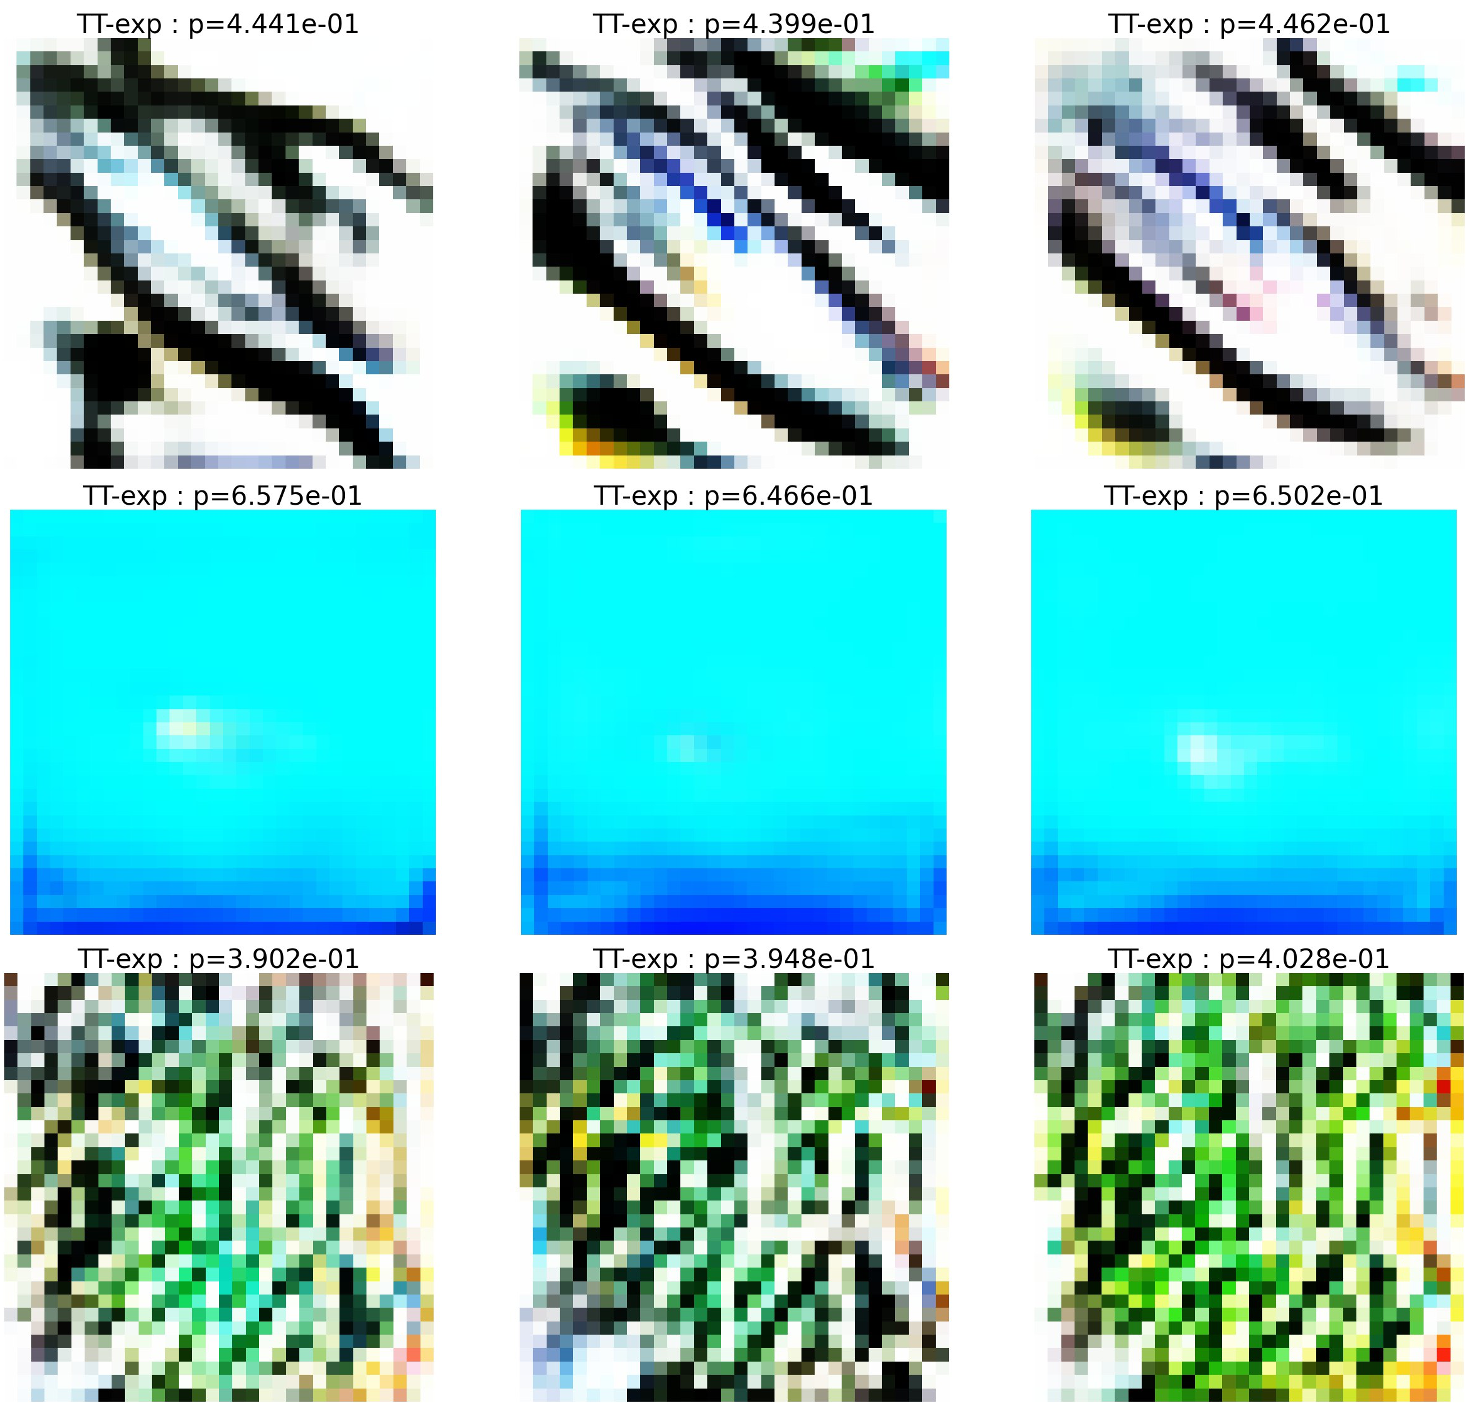
\includegraphics[width=0.8\textwidth]{images/neurotrain/MEI-gallery-0.png}
\caption{MEI нейронов первого импульсного (sn1) слоя. Каждая строка~--- определённый нейрон, несколько оптимумов активации.}
\label{nt:MEI-gallery-0}
\end{figure}

\begin{figure}[ht]
\centering
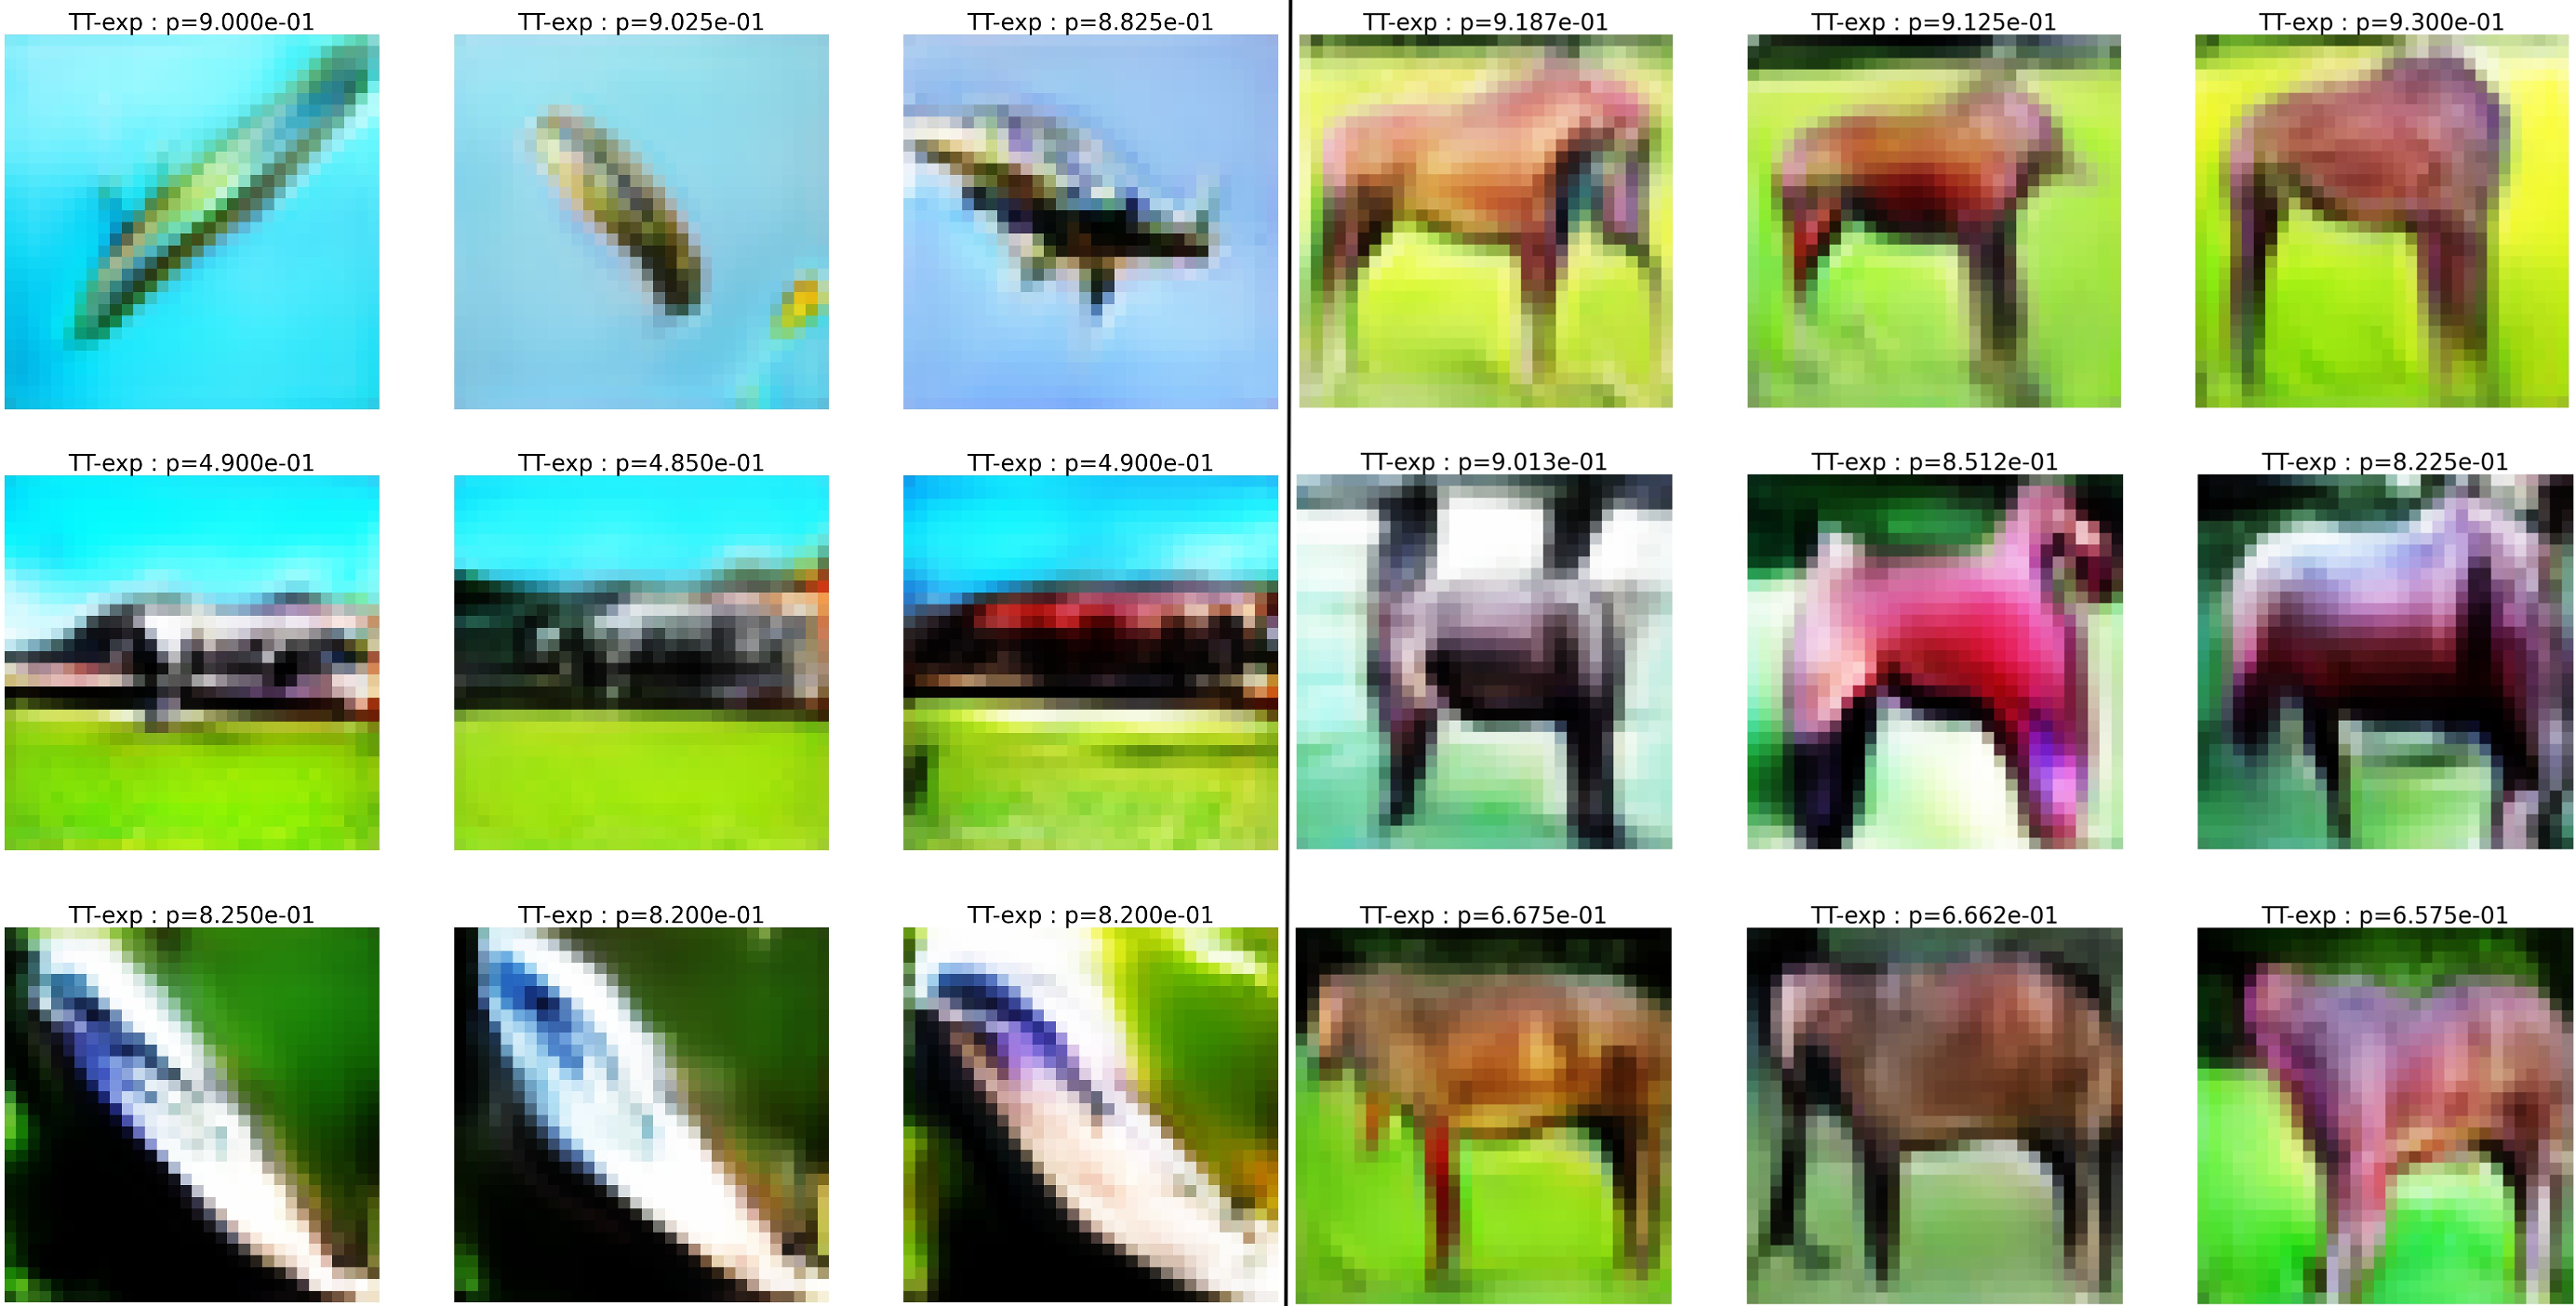
\includegraphics[width=1.0\textwidth]{images/neurotrain/MEI-gallery-1.png}
\caption{MEI нейронов промежуточного (layer2.1.sn1) слоя. Каждые ряды из 3 изображений~--- один нейрон, несколько оптимумов активации. Левый блок $3\times3$~--- 3 разных нейрона с различными специализациями. Правый блок $3\times3$~--- 3 разных нейрона с похожими специализациями.}
\label{nt:MEI-gallery-1}
\end{figure}

\begin{figure}[ht]
\centering
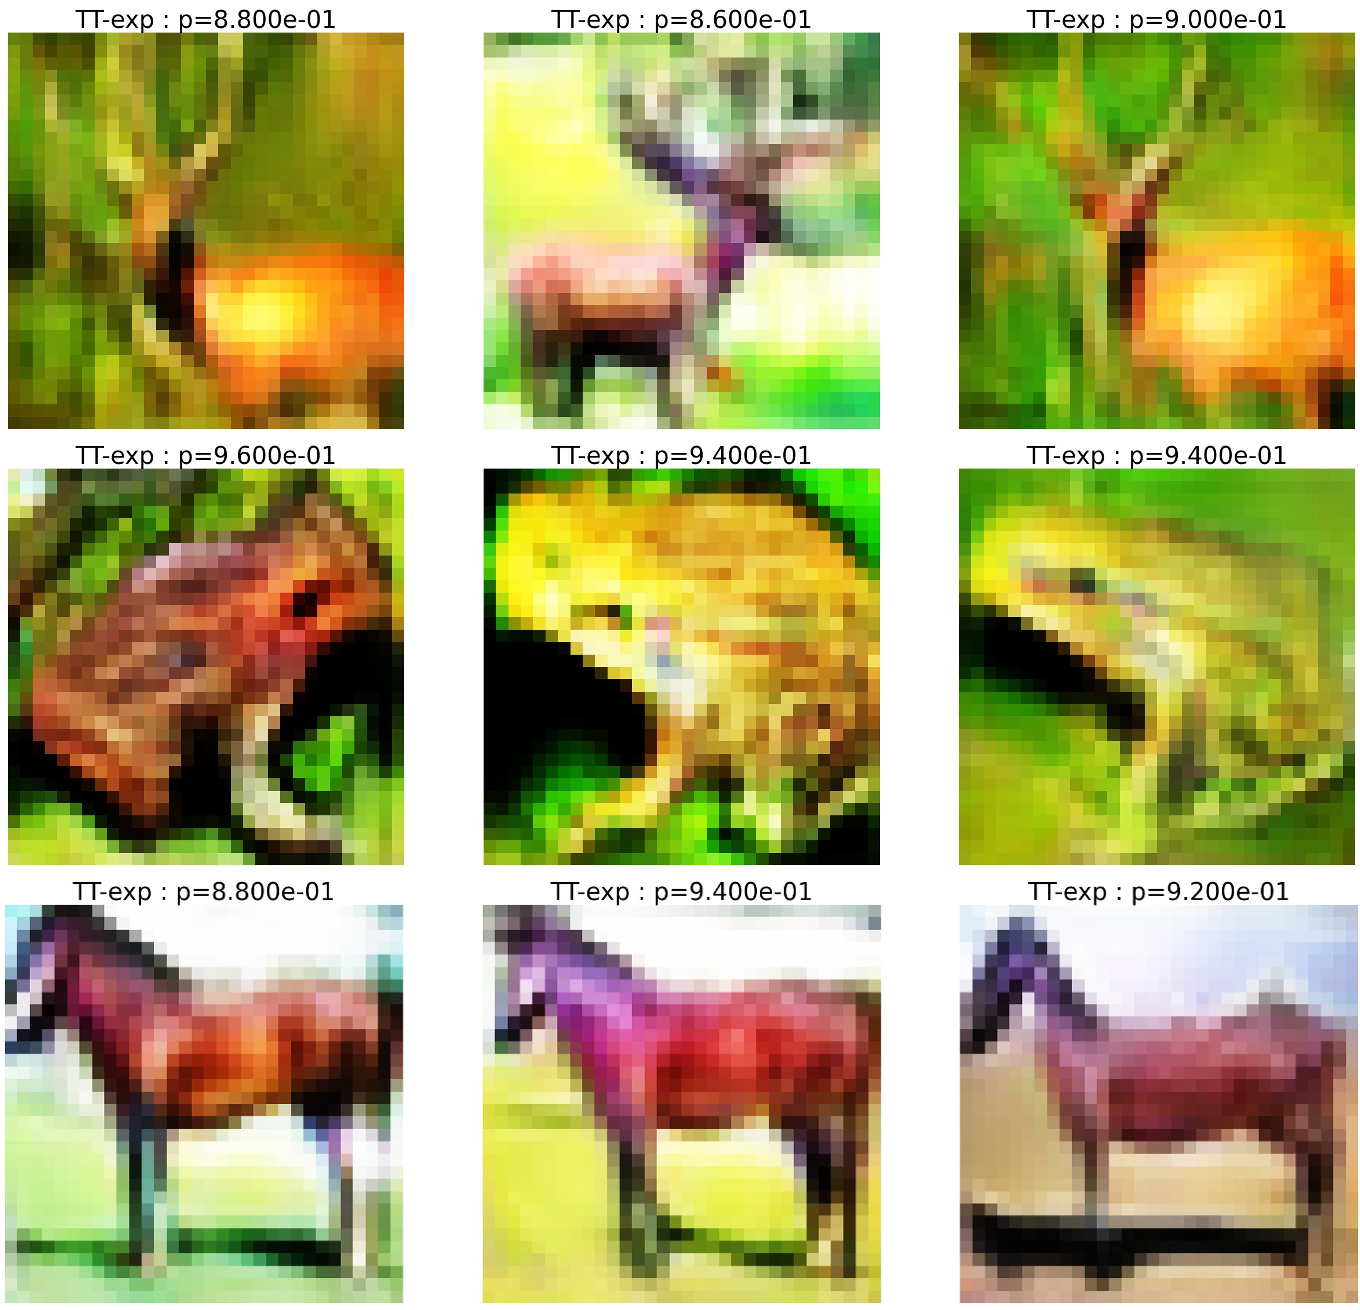
\includegraphics[width=0.8\textwidth]{images/neurotrain/MEI-gallery-2.png}
\caption{MEI последнего импульсного слоя (layer4.1.sn1). Каждая строка~--- определённый нейрон, несколько оптимумов активации.}
\label{nt:MEI-gallery-2}
\end{figure}

\paragraph{Разнообразие MEI.}
MEI, полученные различными методами оптимизации, содержали одни и те же паттерны различной степени сложности, однако не были идентичны друг другу. Для оценки вариабельности полученных изображений были вычислены средние евклидовы и косинусные расстояния между латентными векторами, соответствующими MEI (с использованием генератора SN-GAN).

\begin{figure}[ht]
\centering
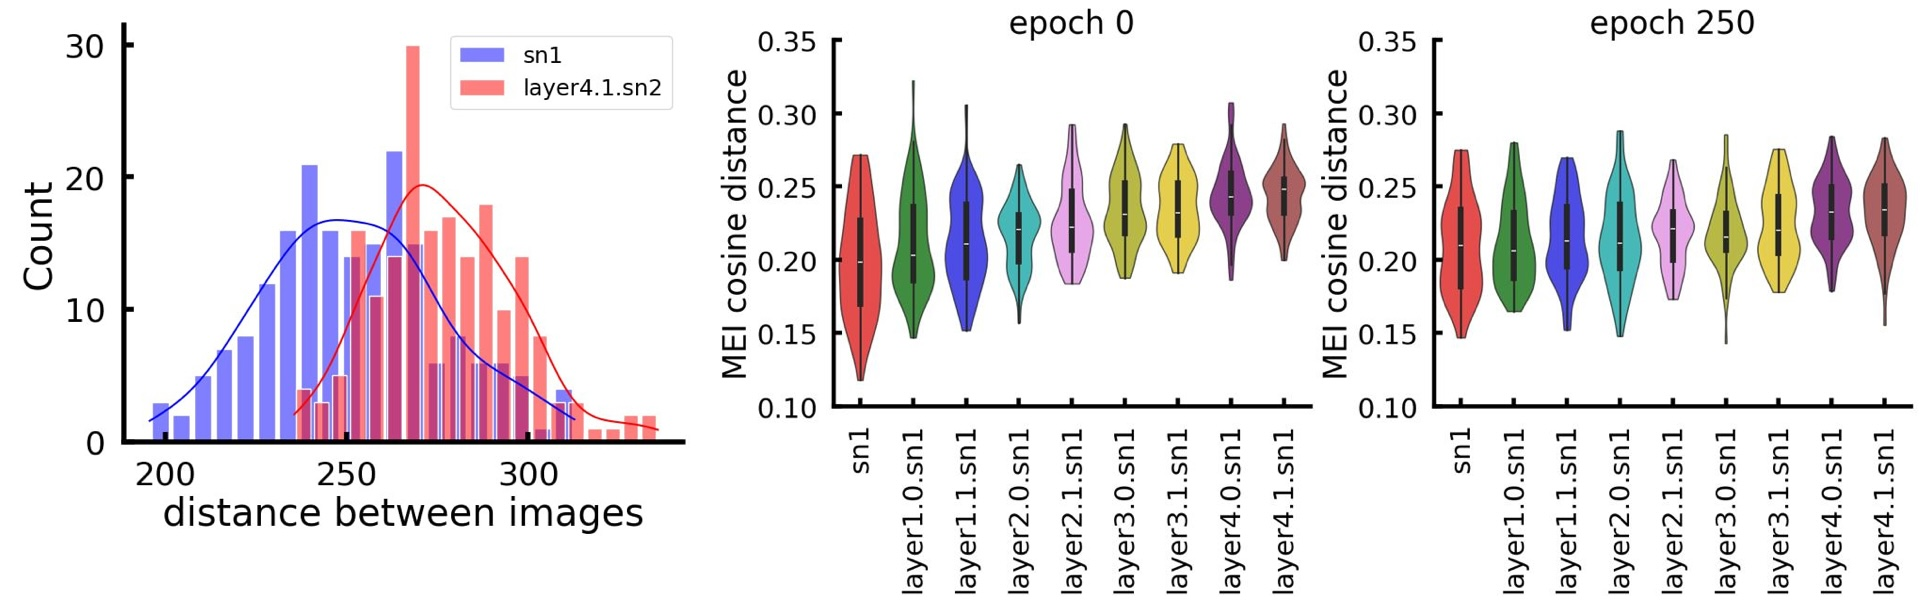
\includegraphics[width=1.0\textwidth]{images/neurotrain/MEI-distances.jpg}
\caption{Разнообразие специализаций с точки зрения расстояний между MEI в латентном пространстве. \textbf{Слева}: евклидовы расстояния. \textbf{Справа}: косинусные сходства для разных слоёв (глубина слоя увеличивается вправо) на разных этапах обучения.}
\label{nt:image-dists}
\end{figure}

Вариабельность MEI в последних слоях импульсной ResNet18 оказалась больше, чем в первых (рис.~\ref{nt:image-dists}). Средние расстояния между сгенерированными MEI в последнем импульсном слое были примерно на 20\% выше, чем в первом, что свидетельствует о значительных трансформациях ландшафта специализаций нейронов. Возможное объяснение этого эффекта состоит в том, что существует множество способов реализации сложной концепции в изображении. Нейронные сети в процессе обучения осуществляют нелинейную проекцию пространства данных, одновременно отождествляя некоторые его области~\cite{nnmap}, в результате чего количество локальных максимумов в общем пространстве изображений растёт с увеличением специализации нейронов. В то же время данный эффект, измеренный через косинусное расстояние, ослабевал по мере обучения модели (рис.~\ref{nt:image-dists}, справа).

Растущее разнообразие MEI сопровождалось увеличением активаций, которые они вызывали на соответствующих нейронах (рис.~\ref{nt:image-acts}), что объясняется более тонкой специализацией нейронов в глубоких слоях. При этом провалы в максимальных значениях активации, наблюдаемые в слое 3.1, воспроизводились обоими типами генераторов (GAN и VAE), что указывает на более сложную общую картину.

\paragraph{Сложность MEI.}
По мере обучения сети содержание MEI становилось более сложным. Вычисление точной меры сложности изображения представляет собой нетривиальную задачу~\cite{Chikhman2012}, однако общее представление можно получить с помощью эвристик, основанных на алгоритмах сжатия информации. Данный подход зарекомендовал себя при оценке энтропии и взаимной информации~\cite{Baronchelli2005}, а также при количественной оценке уровня сознания~\cite{Casali2013}. Для количественной оценки визуальной сложности MEI были вычислены коэффициенты сжатия оптимизированных изображений в форматах \texttt{.jpg} и \texttt{.zip} и проведено сравнение с размером исходных изображений (рис.~\ref{nt:complexity-by-compression}).

\begin{figure}[ht]
\centering
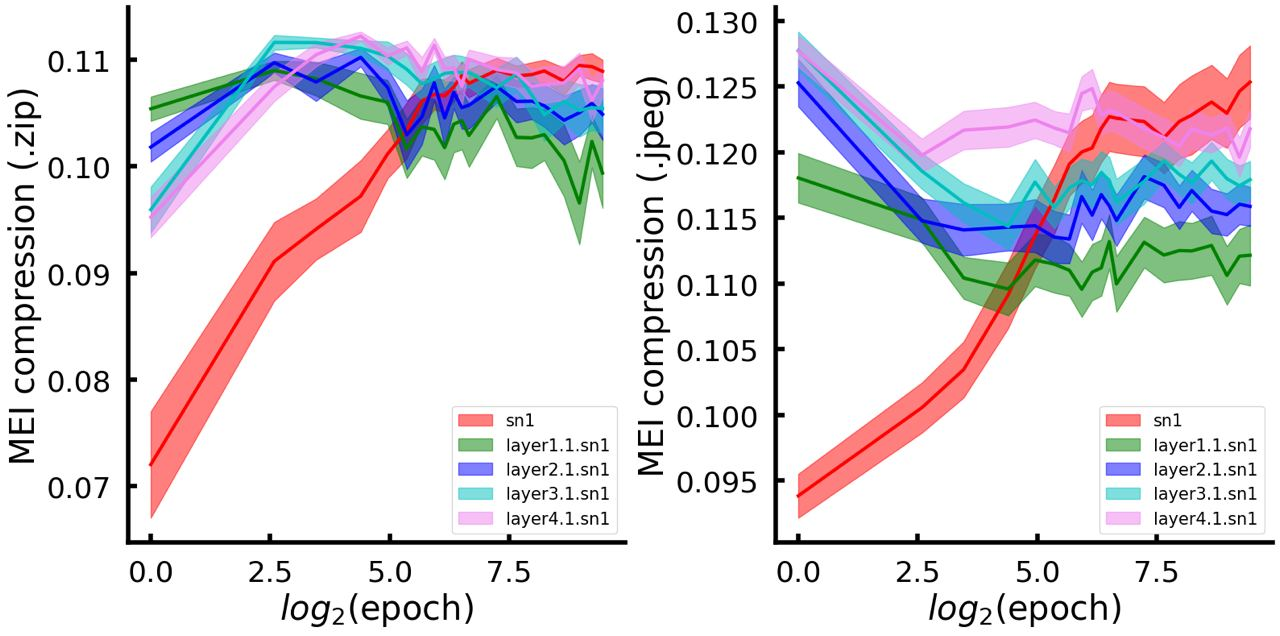
\includegraphics[width=0.95\textwidth]{images/neurotrain/complexity-by-compression.jpg}
\caption{Сложность MEI, измеренная как размер сжатого файла (сжатие JPEG и ZIP).}
\label{nt:complexity-by-compression}
\end{figure}

Оба метода сжатия дали согласованные результаты: по мере обучения сети сложность MEI в первых слоях увеличивалась, постепенно достигая устойчивого состояния. Данный эффект связан с быстрым формированием более сложных специализаций в ранних слоях сети (рис.~\ref{nt:image-acts}).
